\documentclass[12]{article}%12pt即为*四号字
\usepackage{ctex}%引入中文包
\usepackage{graphicx}%插入图片的包
\usepackage{geometry}%设置A4纸页边距的包
\usepackage{url}
\usepackage{stfloats}
\usepackage{float}
\geometry{left=3.18cm,right=3.18cm,top=2.54cm,bottom=2.54cm}%设置页边距
\linespread{1}%设置行间距



\begin{document}
\begin{center}
    \LARGE\songti\textbf{Chapter 4 homework} \\%标题
    \large\kaishu\textbf{褚朱钇恒\qquad 3200104144}%一般是我的姓名
\end{center}
    \section{Theoretical questions}
        \subsection{I}
        result = $1.11011101\times2^8$

        \subsection{II}
        result = $1.001001001\cdots\times2^1$

        \subsection{III}
        $x=1.0000\cdots00\times \beta^e$

        $x_L=(\beta-1).(\beta-1)\cdots(\beta-1)\times \beta^{e-1}$
        $x_R=1.000\cdots1\times \beta^{e-1}$

        So, $x_R-x=\beta^{e-p},x-x_L=\beta^{e-p-1}$

        Then we have $x_R-x=\beta(x-x_L)$
        
        \subsection{IV}
        $x_L=1.00100100100100100100100\times2^{-1},x_R=1.00100100100100100100101\times 2^{-1}$

        $fl(x)=x_R$,roundoff error $=\frac{|x_R-x|}{|x|}\approx2^{-25}$
        
        \subsection{V}
        $\epsilon_u=\beta^{-p}=2^{-23}$

        \subsection{VI}
            $cos(0.25)=1.111100000001\cdots\times 2^{-1}$

            $1-cos(0.25)=0.00001\cdots\times 2^{-1}$, so it has 5 bits of precision lost.

        \subsection{VII}
            \begin{enumerate}
                \item $1-cos(x)=1-(1-\frac{x^2}{2!}+\frac{x^4}{4!}\cdots)=\frac{x^2}{2!}-\frac{x^4}{4!}\cdots$
                \item $1-cos(x)=2sin^2(\frac{x}{2})$
            \end{enumerate}

        \subsection{VIII}
            \begin{enumerate}
                \item $f(x)=(x-1)^\alpha,C_f(x)=|\frac{\alpha x(x-1)^{\alpha-1}}{(x-1)^\alpha}|$,if $\alpha\neq0$,$C_f$ is large when $ x\rightarrow 0$
                \item $f(x)=ln(x),C_f(x)=|\frac{1}{ln(x)}|$,$C_f$ is large when $ x\rightarrow 0$
                \item $f(x)=e^x,C_f(x)=|x|$,$C_f$ is large when $ x\rightarrow \infty$
                \item $f(x)=arccos(x),C_f(x)=|\frac{x}{\sqrt{1-x^2}arccos(x)}|$,$C_f$ is large when $ x\rightarrow \pm 1$
           
            \end{enumerate}

        \subsection{IX}
            \begin{enumerate}
                \item $C_f(x)=\frac{x}{1+e^x},\forall x\in[0,1 ]$
                \item $C_A(x)=\frac{1}{\epsilon_u}\inf_{x_A}\frac{|x_A-x|}{|x|}$
                    
                        $f^{'}(x)=e^{-x}\ge \frac{1}{e}$

                        $|f(x_A)-f(x)|=f^{'}(\xi)|x_A-x|\le \epsilon_u$

                        So,$|x_A-x|\le e\epsilon_u$

                        Then $C_A(x)\le \frac{e}{|x|}$
                \item $C_f (x)$ and the estimated upper bound of $C_A(x)$ as a function of x on [0, 1] is showed by the picture:
            \end{enumerate}
            \begin{figure}[H]
                \centering
                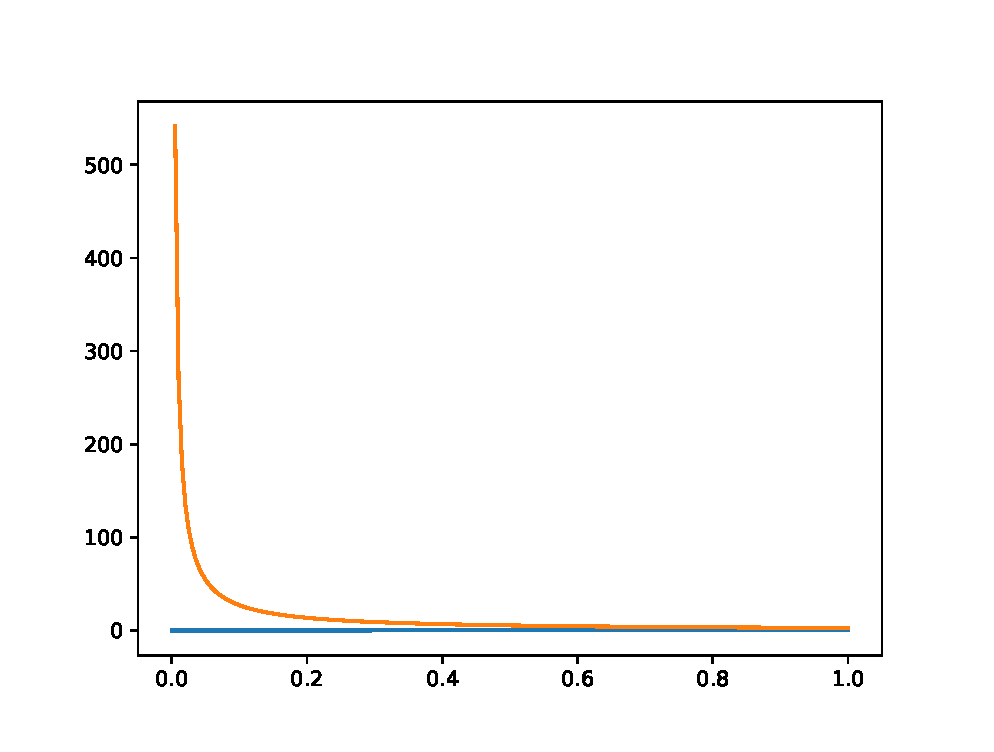
\includegraphics[width=0.7\textwidth]{./pic/IX.eps}
                \caption{$C_f$ and $C_A$ on $[0, 1]$}
            \end{figure}

                when $x=0$, $f(0)=0,f_A(x)=f(x)(1+\delta(x))$, $\delta(x)\rightarrow \infty$.

                So $x\rightarrow 0,C_A(x)\rightarrow \infty$

        \subsection{X}
            $Cond_1=|\frac{1}{r}|\Sigma_{i=0}^{n-1}|a_i\frac{\partial r}{\partial a_i}|=\frac{\Sigma_{i=0}^{n-1}|a_ir^i|}{r(\Sigma_{i=1}^{n}(n-i+1)a_ir^{n-i})}$

            Let $r=n,f(x)=\Pi_{i=1}^n(x-i)$, then we have $Cond_1\ge\frac{n^n}{n!}$

            When n is large ,$Cond_1$ also become very large, which is consistent with the Wilkinson.

        \subsection{XI}
            In FPN system(10,1,-1,1),$\frac{4}{9}=0.44444=0$

            $\frac{0-\frac{4}{9}}{\frac{4}{9}}=1>\epsilon_u$

        \subsection{XII}
            对$x\in[128,129]$,$x=m\times 2^e,e=7$.

            所以区间内两个相邻浮点数的距离为$2^7\epsilon_M=2^{-16}>10^{-6}$

            所以不能将计算根的精度降低到$1e-6$
        
        \subsection{XIII}
            设$x_i,x_{i+1}$的距离很近,即$|x_i-x_{i+1}|\le \delta$

            则计算三次样条$p(x)=a+b(x-x_i)+c(x-x_i)^2+d(x-x_i)^3$的方程为:

            \begin{displaymath}
                \left( \begin{array}{cccc}
                    1 & 0 & 0& 0\\
                    1 & \delta&\delta^2&\delta^3\\
                    0 & 1 & 0 & 0\\
                    0 & 1 & 2\delta &3\delta
                 \end{array} \right)
                 \left( \begin{array}{cccc}
                    a\\
                    b\\
                    c\\
                    d
                 \end{array} \right)=
                 \left( \begin{array}{cccc}
                    f(x_i)\\
                    f(x_{i+1})\\
                    f^{'}(x_i)\\
                    f^{'}(x_{i+1})
                 \end{array} \right)
            \end{displaymath}

            当$\delta$小时,方程组的条件数极大,故此时三次样条结果不稳定。
\end{document} 